\chapter{Circuit Schematics}
%\comment{
\begin{landscape}
	\begin{figure}[hbtp]
		\centering
		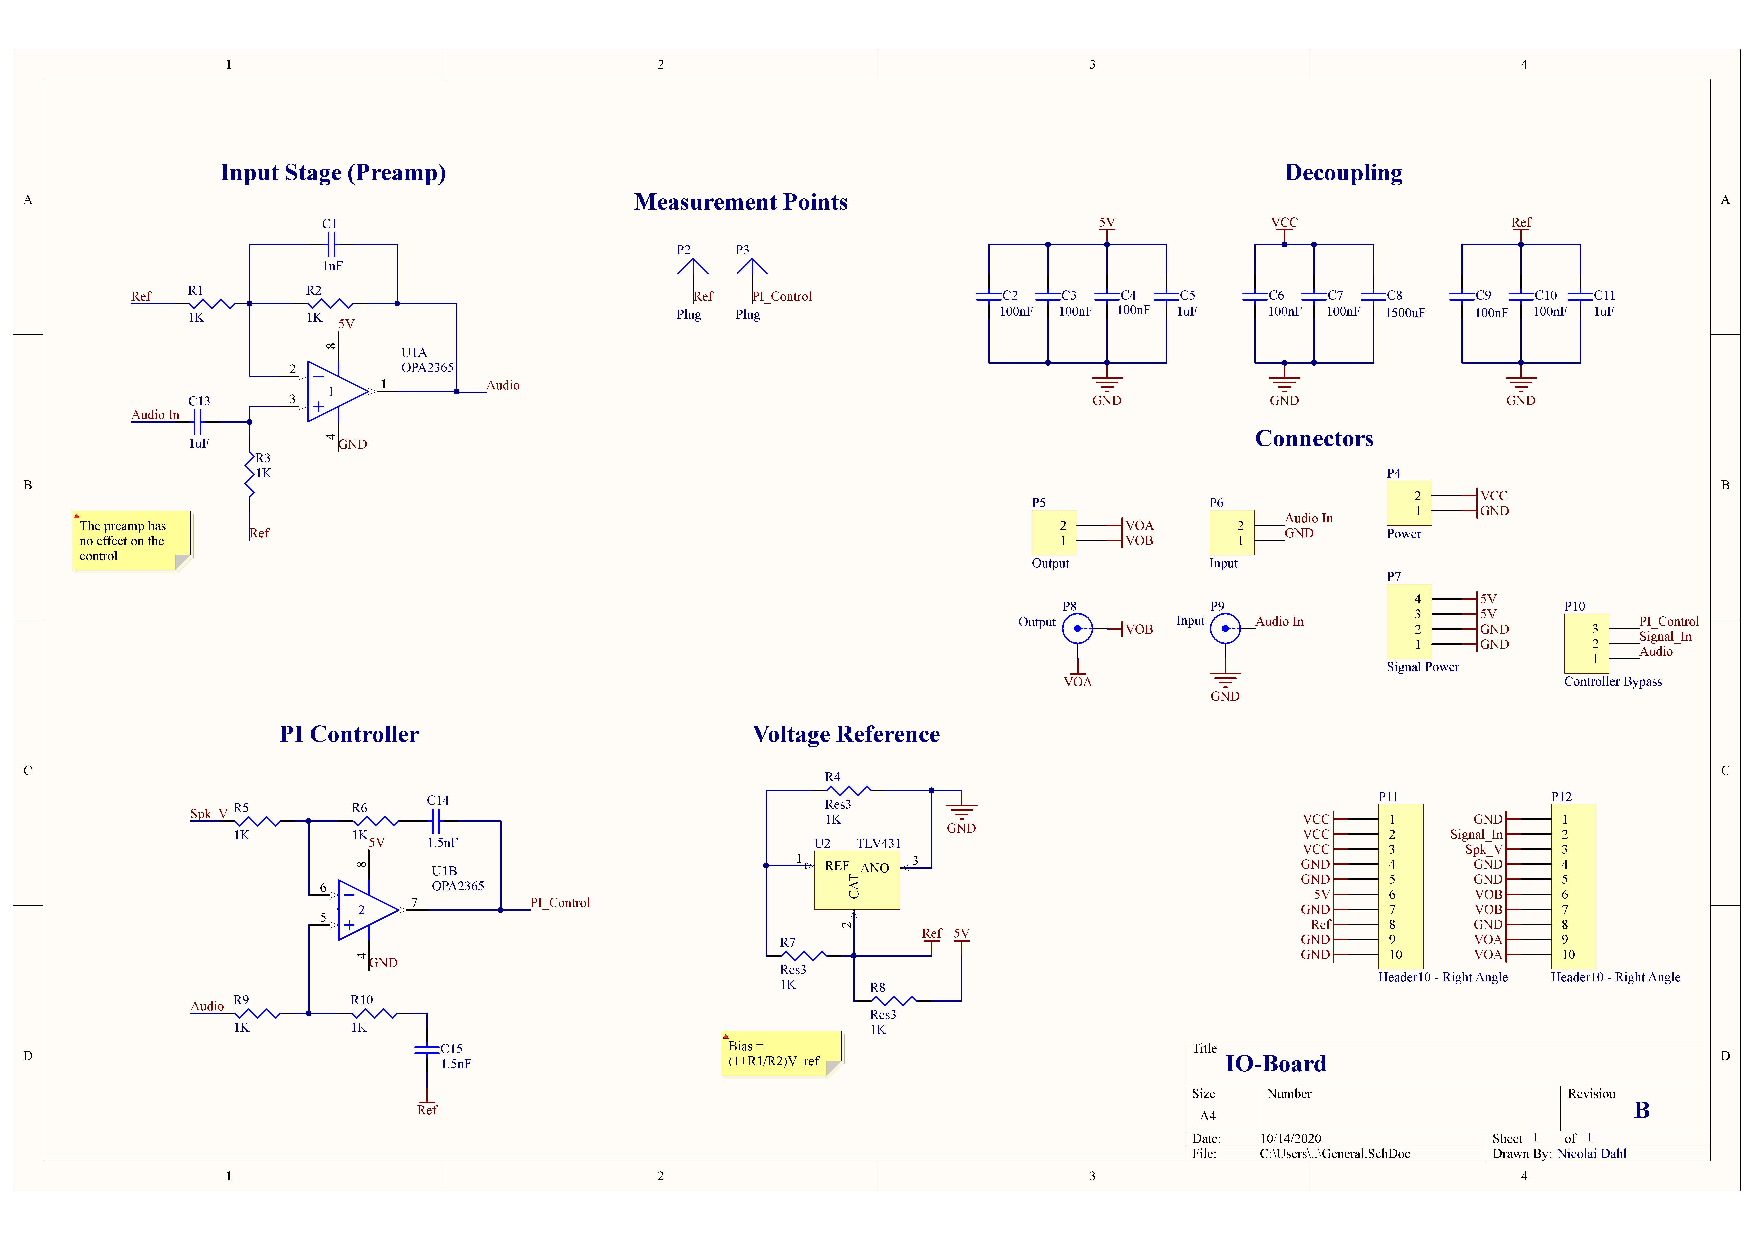
\includegraphics[width=20cm,height=28.7cm,keepaspectratio]{0_Figures/Appendix/IO_Board_Schematic.pdf}
		\caption{Schematic of IO Board \cite{multivar_ctrl_loops_for_SM_audio_systems}}
		\label{fig:schematic_io_board}
	\end{figure}
\end{landscape}
\clearpage
\begin{landscape}
	\begin{figure}[hbtp]
		\centering
		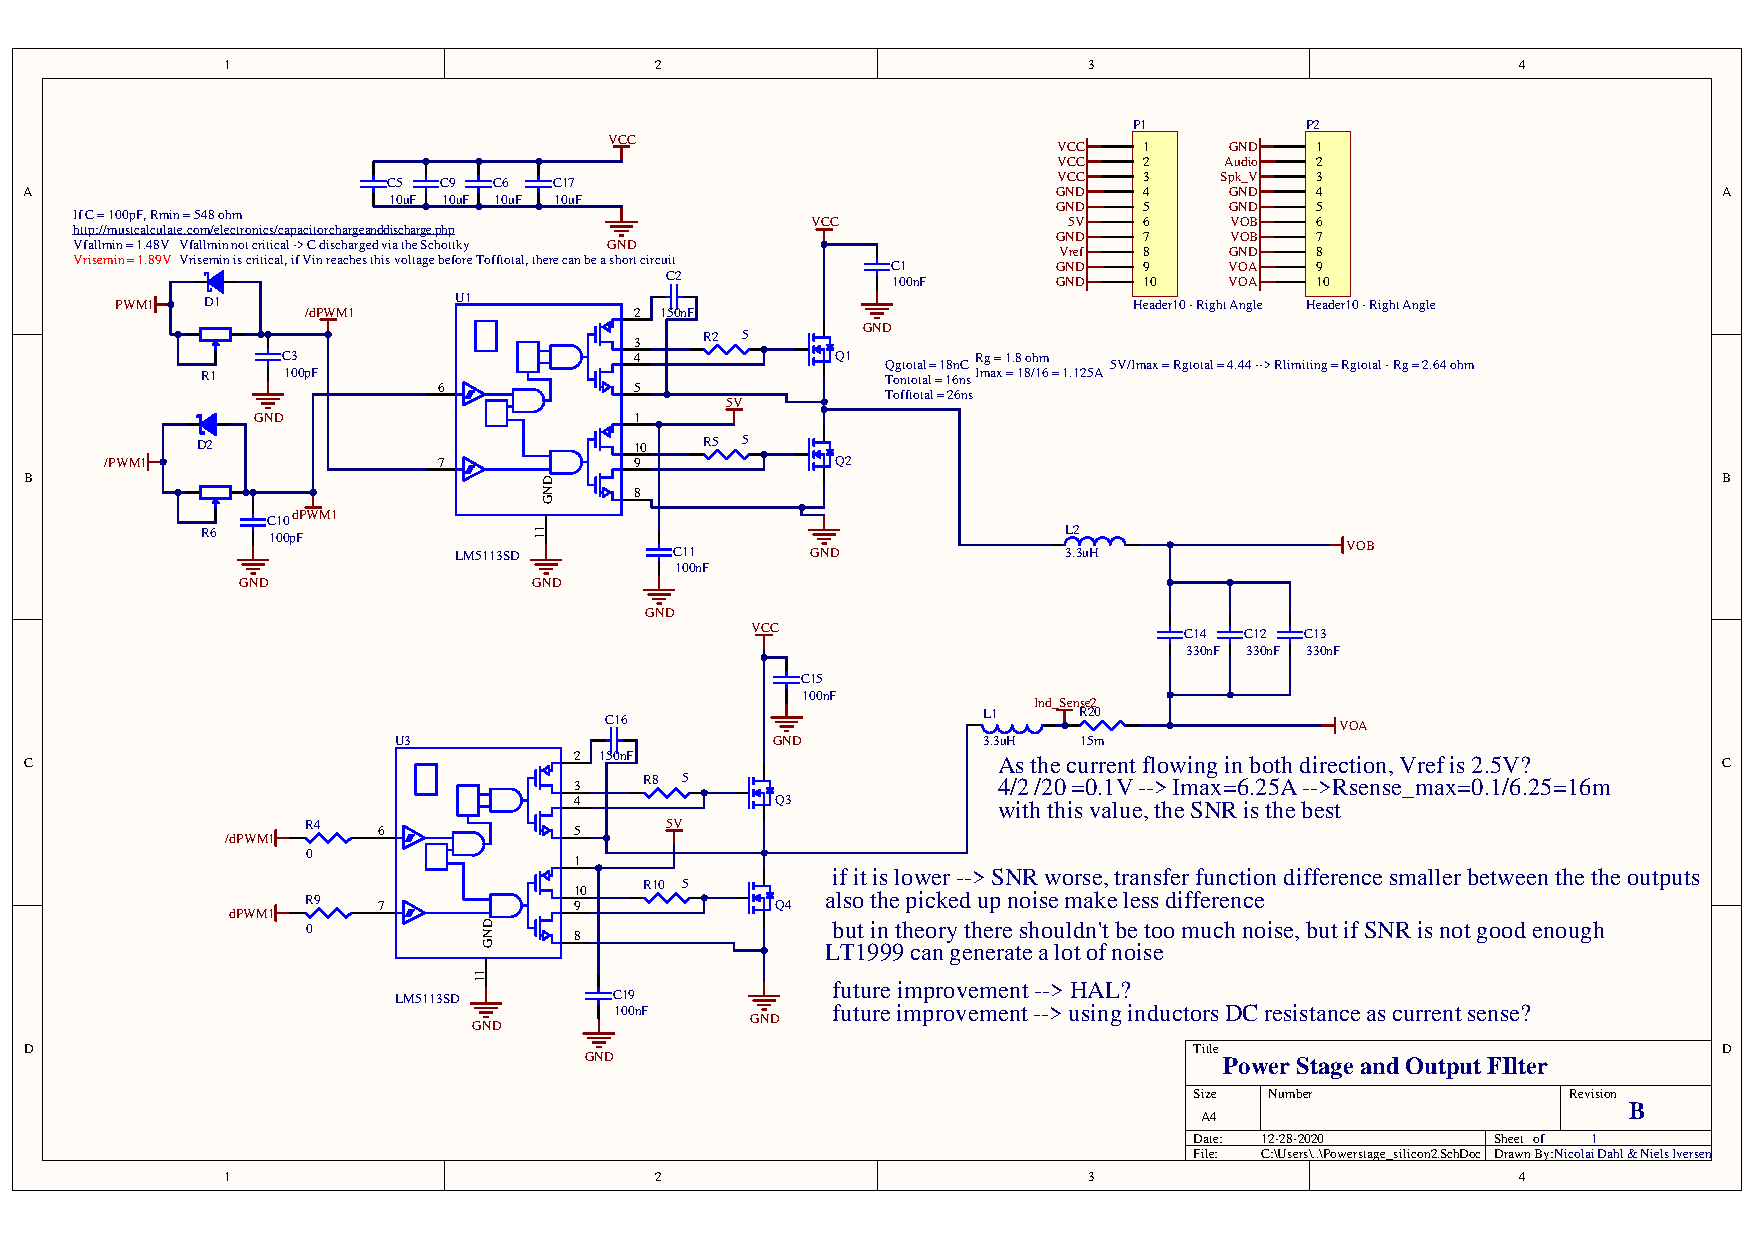
\includegraphics[width=20cm,height=28.7cm,keepaspectratio]{0_Figures/Appendix/Power_Stage_Schematic.pdf}
		\caption{Schematic of Power Stage \cite{multivar_ctrl_loops_for_SM_audio_systems}}
		\label{fig:schematic_power_stage}
	\end{figure}
\end{landscape}
\clearpage
\begin{landscape}
	\begin{figure}[hbtp]
		\centering
		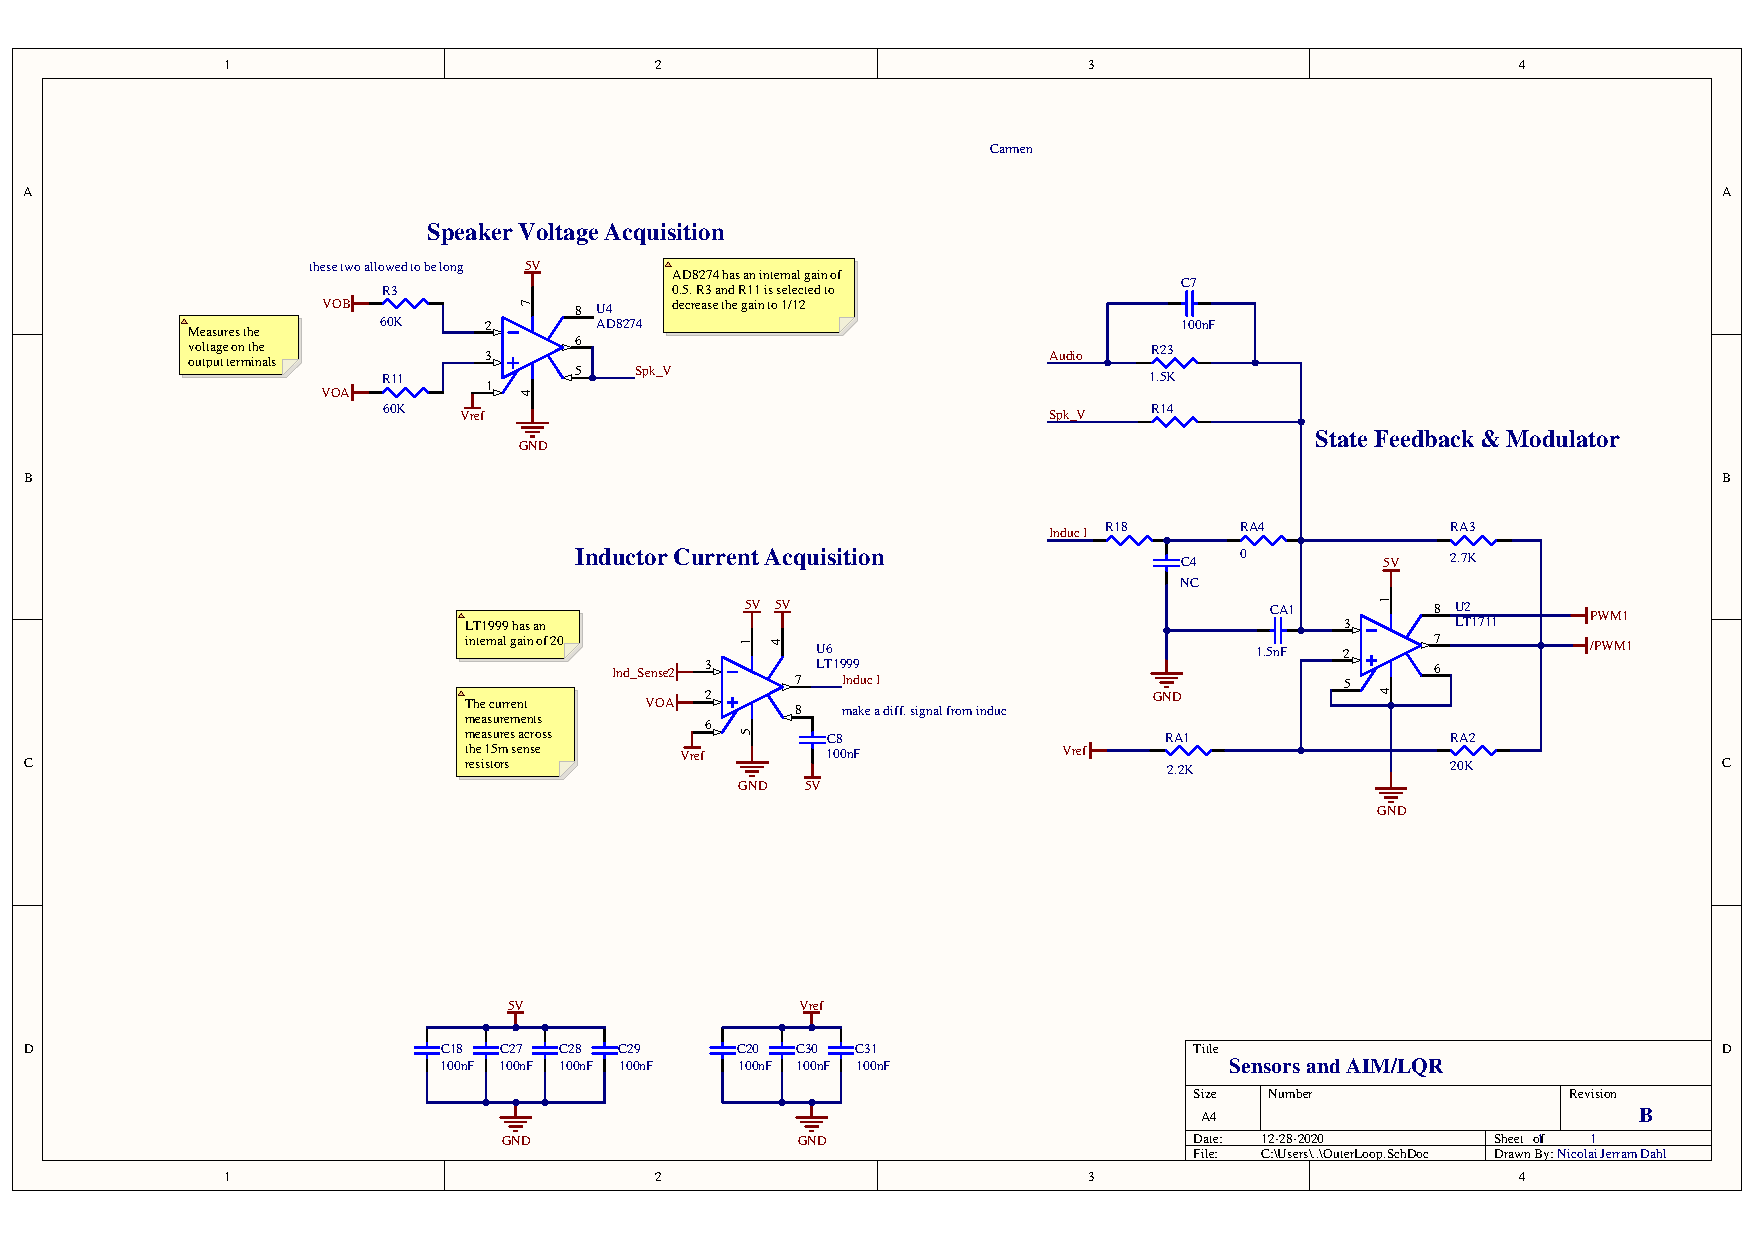
\includegraphics[width=20cm,height=28.7cm,keepaspectratio]{0_Figures/Appendix/OuterLoop_Schematic.pdf}
		\caption{Schematic of Outer Loop \cite{multivar_ctrl_loops_for_SM_audio_systems}}
		\label{fig:schematic_outerloop}
	\end{figure}
\end{landscape}
%}

\chapter{Measurement setups}
\begin{figure}[H]
	\centering
	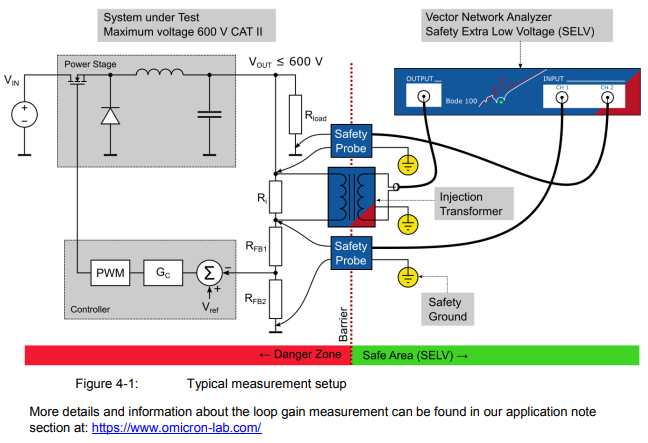
\includegraphics[width=0.9\textwidth]{Appendix/injection_transformer_measurement_setup.png}
	\caption{Typical measurement set-up of injection transformer in feedback loop from user manual \cite{injection_transformer_manual}}
	\label{fig:injection_transformer_setup}
\end{figure}

\begin{figure}[H]
	\centering
	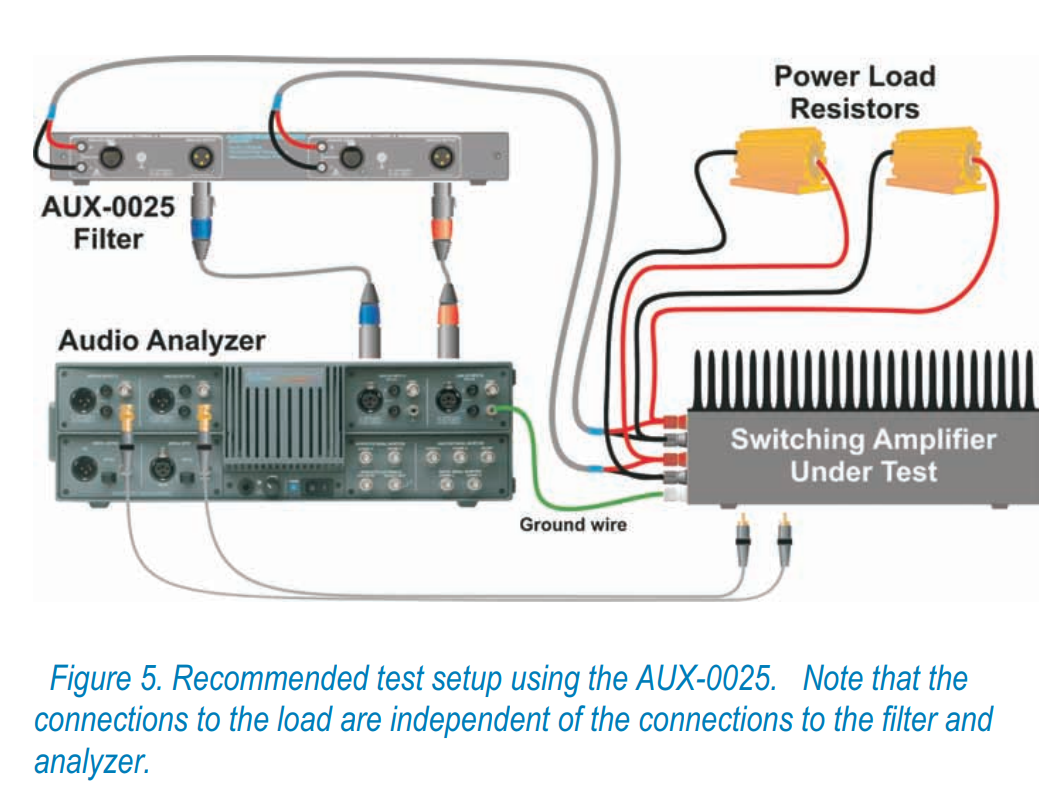
\includegraphics[width=0.9\textwidth]{Appendix/apx500_measurement.png}
	\caption{Typical measurement set-up of Audio Precision APx500 audio analyzer from white paper \cite{apx500_sw_mode_meas}}
	\label{fig:apx500_typical_measurement}
\end{figure}

\chapter{LTspice}

\begin{figure}[H]
	\centering
	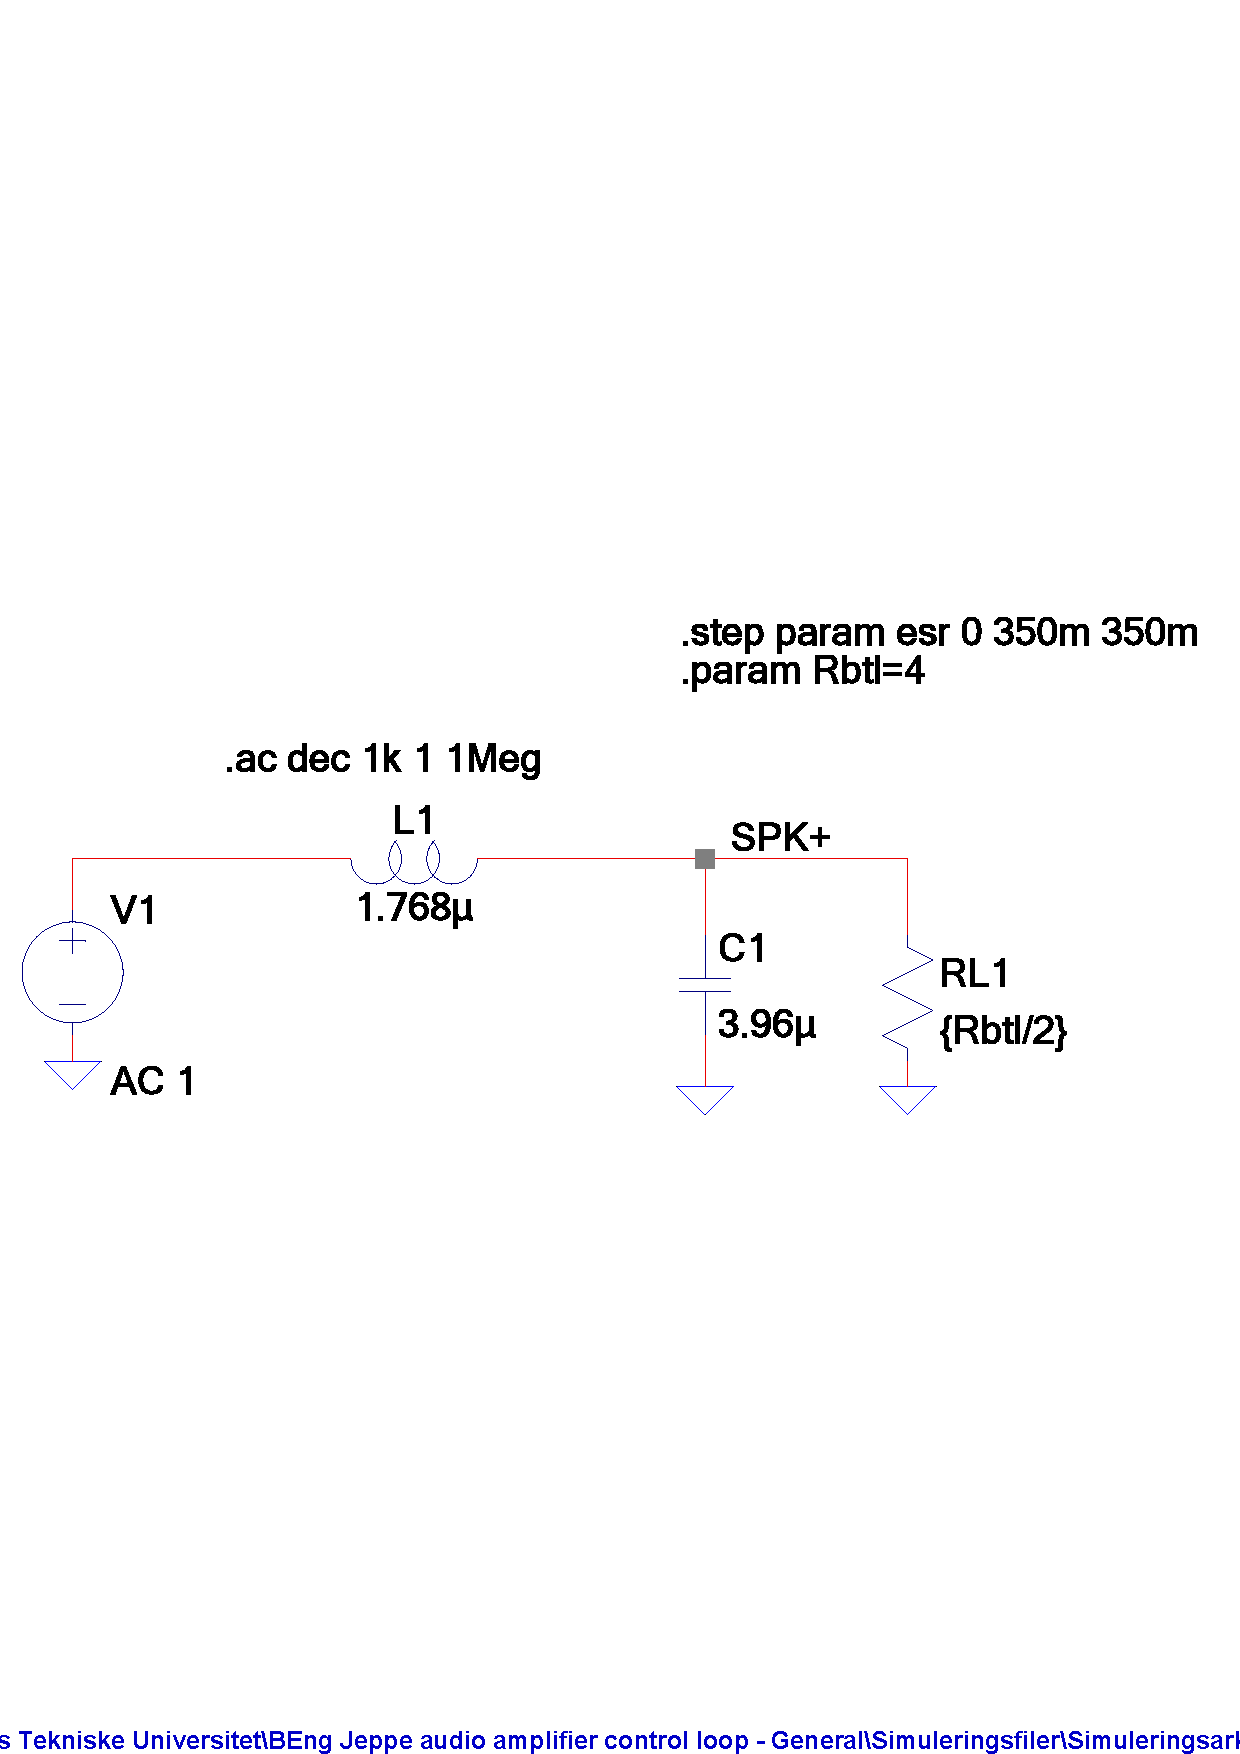
\includegraphics[width=0.6\textwidth, trim=10 210 10 210, clip]{Appendix/ltspice_output_filter.pdf}
	\caption{Small signal analysis of output filter}
	\label{fig:ltspice_output_filter}
\end{figure}

\begin{figure}[H]
	\centering
	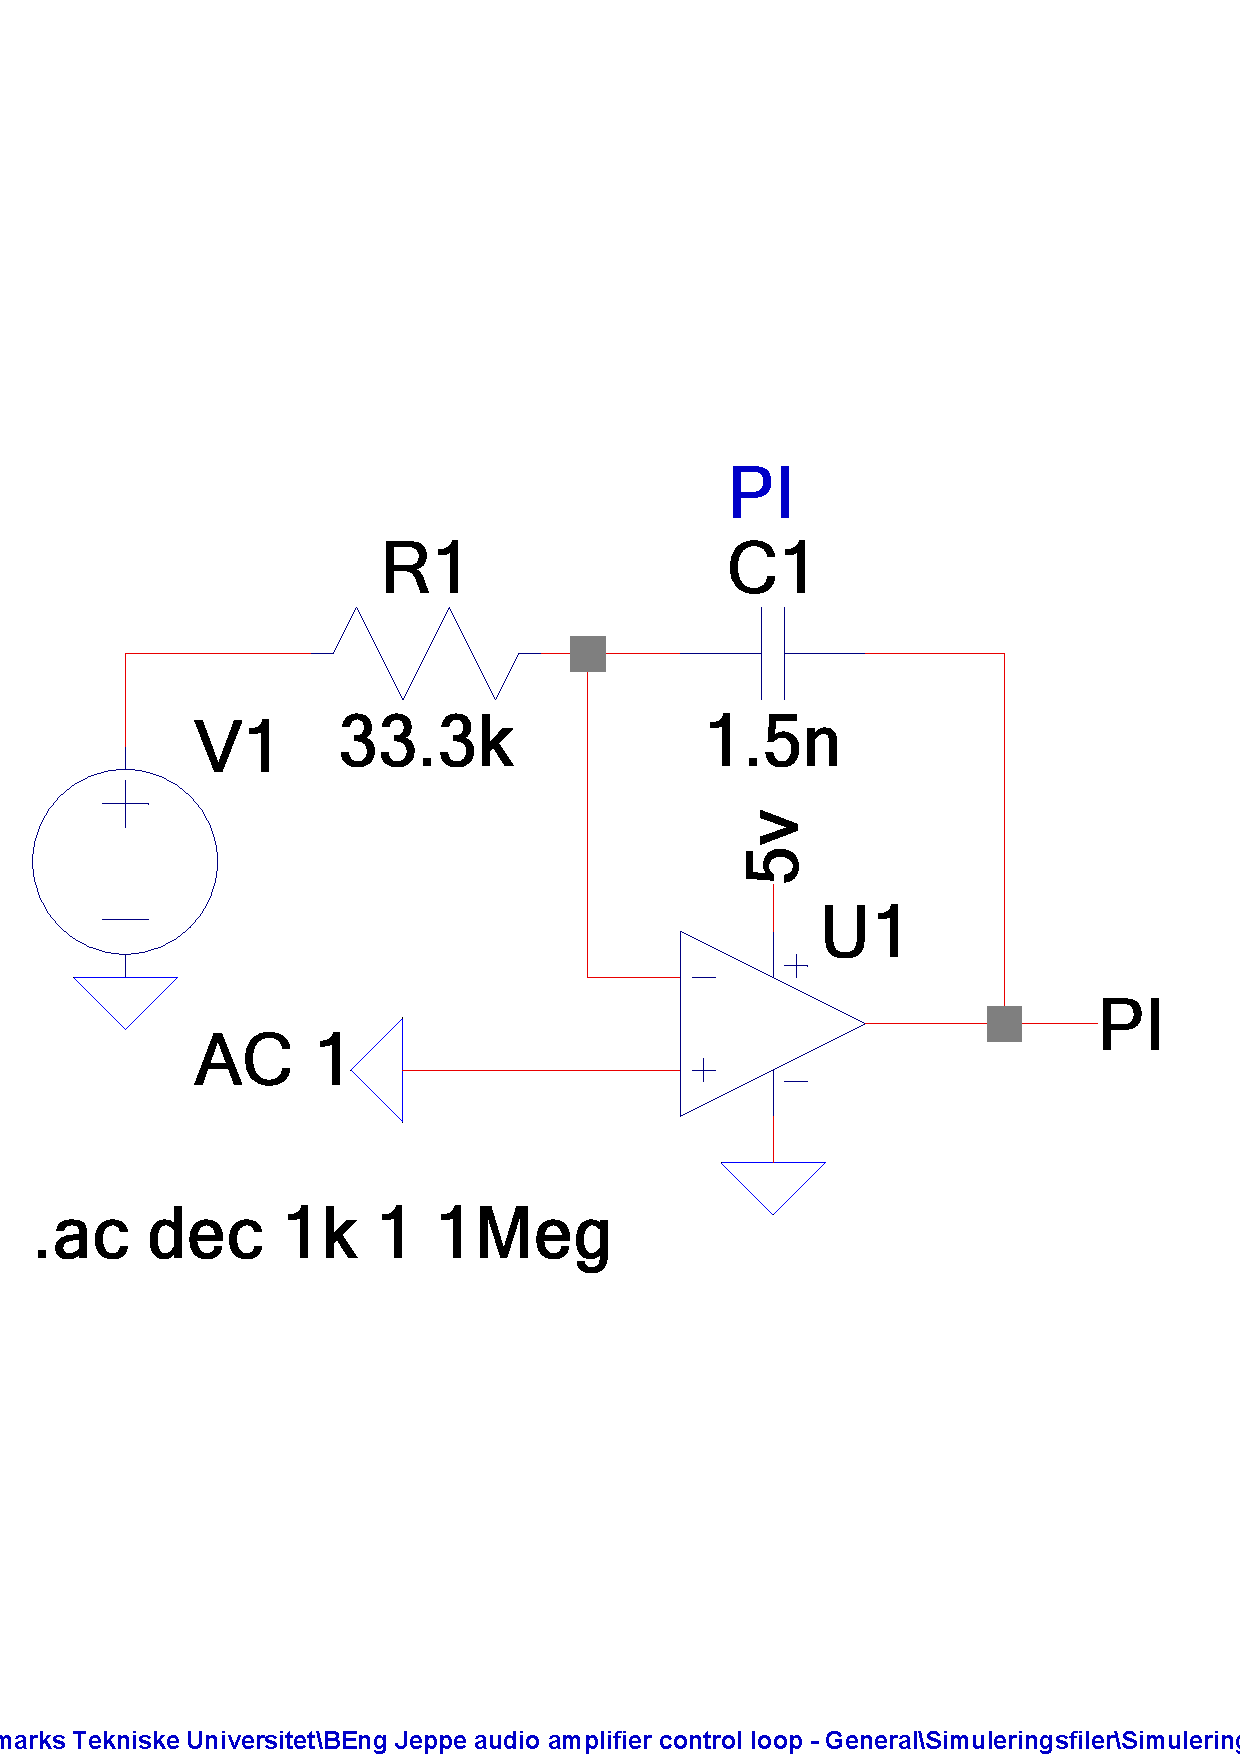
\includegraphics[width=0.4\textwidth, trim=15 210 30 210, clip]{Appendix/ltspice_pi_regulator_ac.pdf}
	\caption{Small signal analysis of PI controller}
	\label{fig:ltspice_pi_regulator_ac}
\end{figure}

\begin{figure}[H]
	\centering
	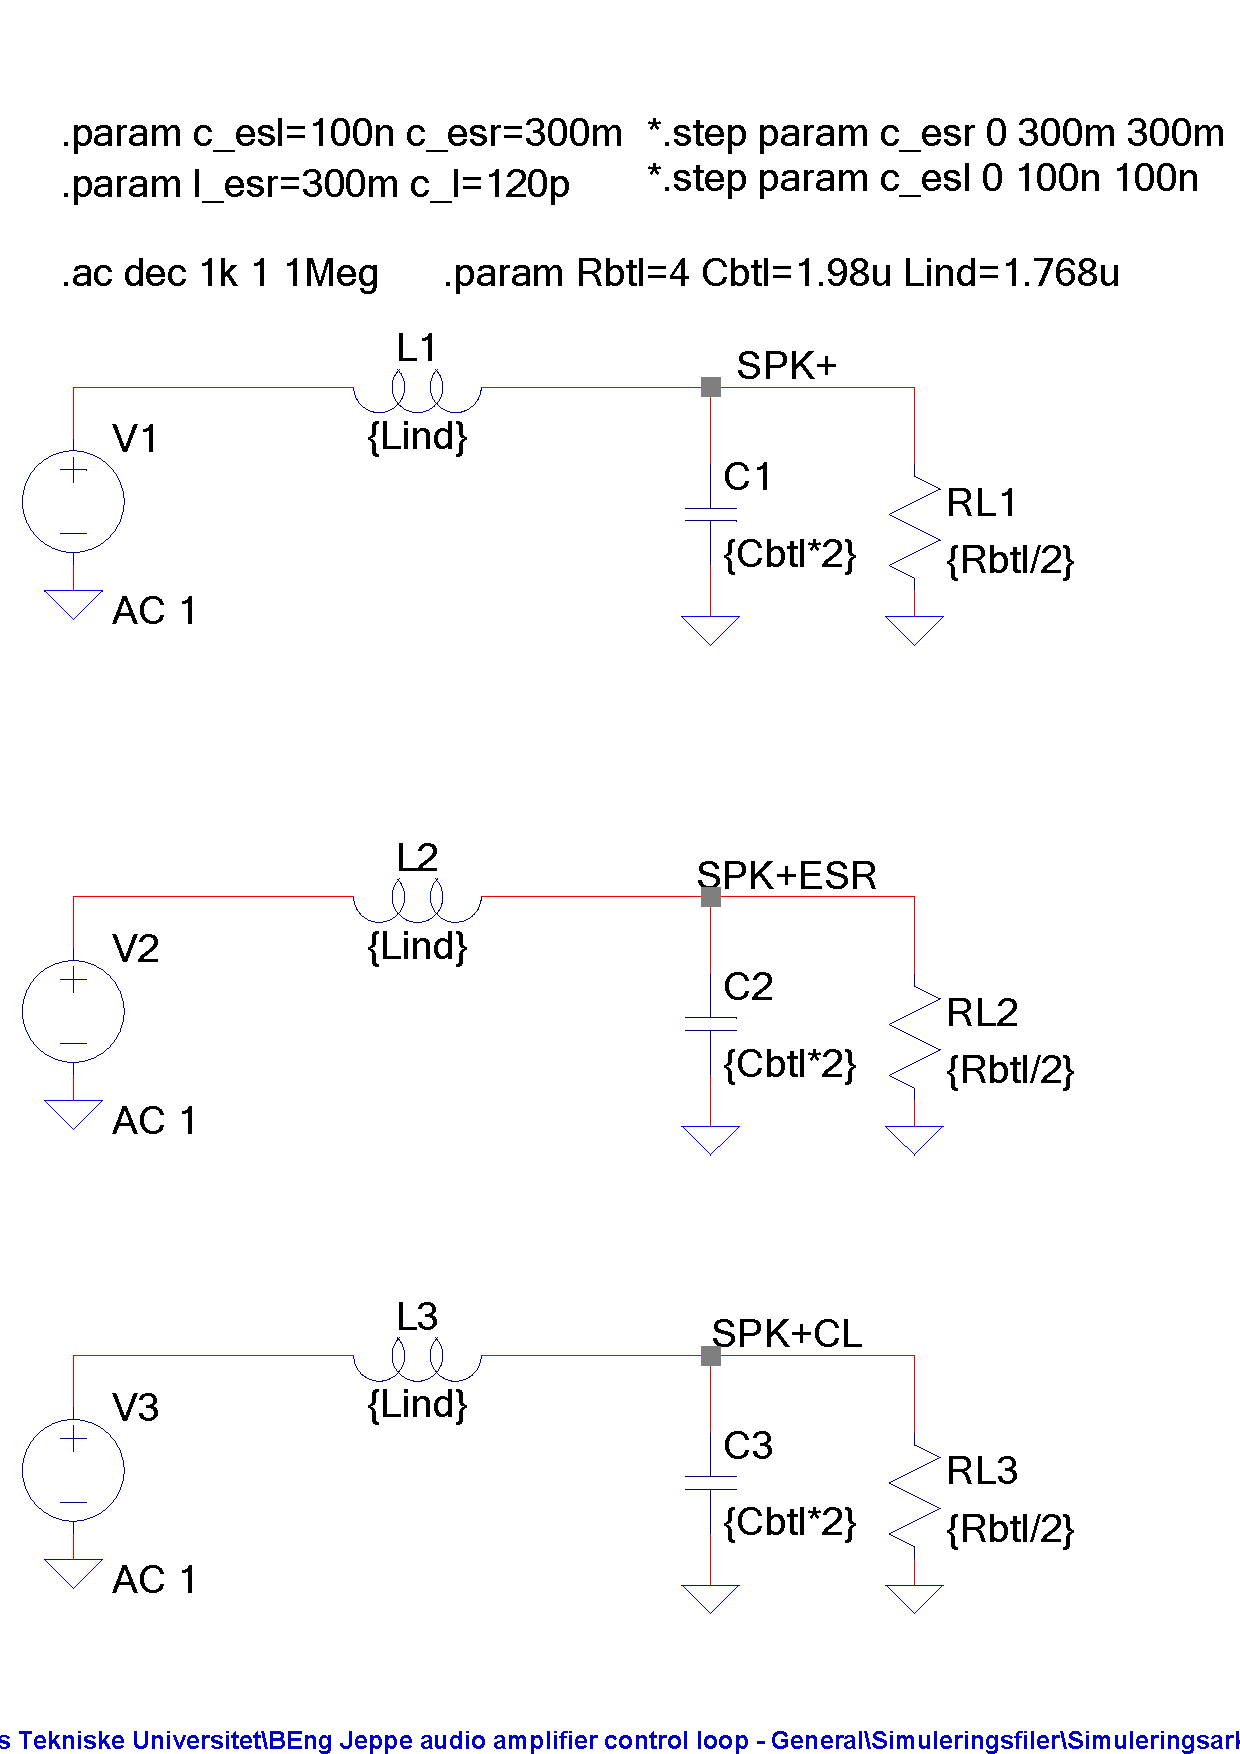
\includegraphics[width=0.6\textwidth, trim=0 50 0 50, clip]{Appendix/ltspice_output_filter_smallsignal.pdf}
	\caption{Small signal analysis of output filter parasitic elements}
	\label{fig:ltspice_output_filter_smallsignal}
\end{figure}

\begin{figure}[htbp]
	\centering
	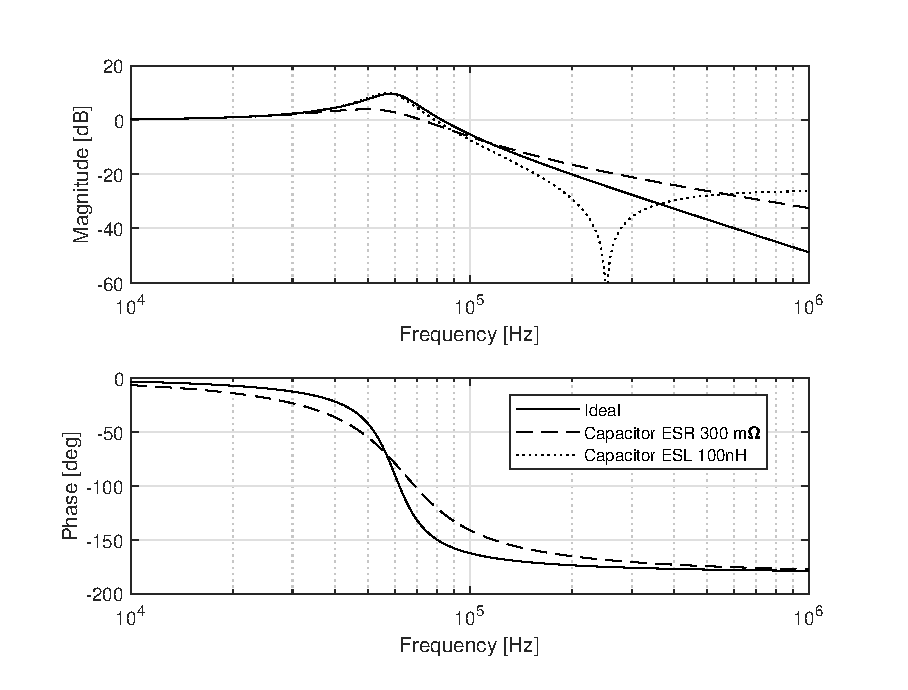
\includegraphics[width=0.6\textwidth]{Appendix/ltspice_output_filter_c_parasitic.eps}
	\caption{Bode plot of output filter using ideal LC filter, parasitic elements in capacitor}
	\label{fig:ltspice_output_filter_c_parasitic}
\end{figure}

It is noted that adding series resistance and inductance to the output capacitor results in a deviating magnitude and higher roll-off at around \SI{-25}{\decibel} in the stopband of high frequency compared to both other curves. To determine the amplitude gain: $$10^{\frac{\SI{-25}{\decibel}}{10}} = \SI{5.6}{\percent}$$ meaning \SI{5.6}{\percent} of the signal is preserved on control loop that returns to the input. Based on this initial hypothesis, it is theorised that parasitic elements in the output capacitor have the greatest altering effect on the transfer function of the control loop.

\chapter{Amplifier analysis}

\section{Efficiency (Simulation)}
To assess the efficiency of the system, an analysis is performed by measuring the power being drawn from the supply and comparing it with the power being delivered to the load. The means is to calculate the efficiency $\eta$, where:
\begin{equation} \label{eq:eff_formula}
	\eta = \frac{P_{\mathrm{out}}}{P_{\mathrm{in}}}
\end{equation}

This is undertaken by implementing a set of SPICE parameters in the simulation, where:
\begin{subequations}
	\begin{equation} \label{eq:eff_power_in}
		P_{\mathrm{in}} = P_{\mathrm{E1}} + P_{\mathrm{E2}} 
	\end{equation}
	\begin{equation} \label{eq:eff_power_out}
		P_{\mathrm{out}} = V_{\mathrm{R_{\mathrm{BTL}}}} \cdot I_{R_{\mathrm{BTL}}}
	\end{equation}
\end{subequations}
In \Cref{eq:eff_power_in}, the sources $E1$ and $E2$ is the power stage voltage supply, a source from each half-bridge. In \Cref{eq:eff_power_out}, the voltage across the load in the bridge-tied-load is multiplied by the current through the bridge-tied-load, it provides the output power. Analysed across an output power sweep it yields the following results:

\begin{figure}[htbp]
	\centering
	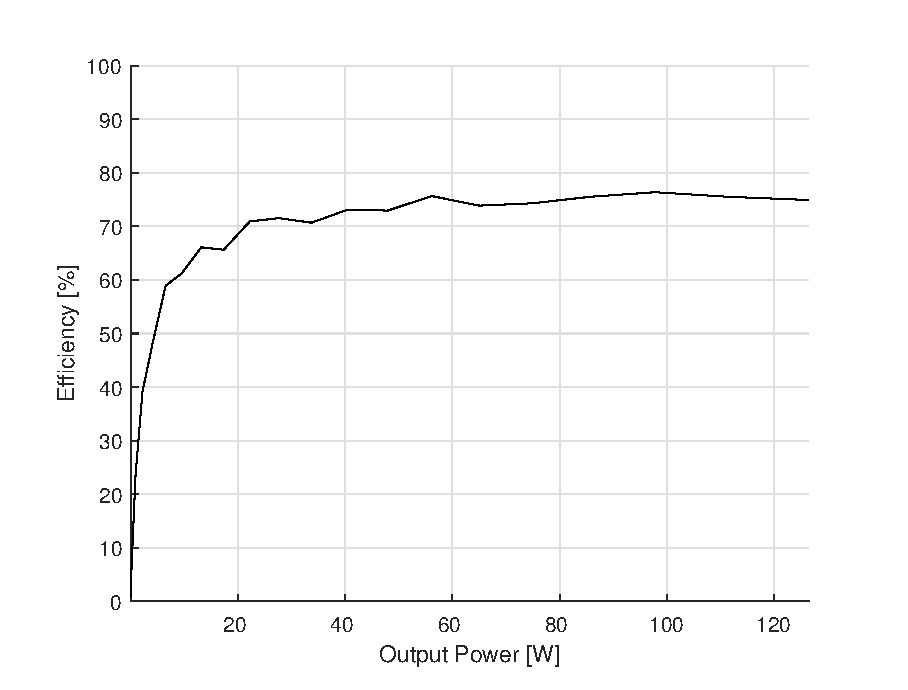
\includegraphics[width=0.8\textwidth]{Analysis/ltspice_eff.eps}
	\caption{Amplifier efficiency across a varying output power}
	\label{fig:eff_output_power}
\end{figure}

As seen in \autoref{fig:eff_output_power}, there is a rather low efficiency in the low output power range, but as the output power increases, the efficiency increases accordingly. Plotted are amplifier with inductor ESR used in the differential filter output from the control loop measurements. The output power seems to taper off at around \SI{75}{\percent}, also a somewhat low efficiency for a class-D amplifier. However, as the serial resistance of the inductor, from an efficiency standpoint, is unreasonably large. It is seen that it would impact the power stage substantially in regards to the efficiency of the amplifier. One thing to note, however, is that this analysis does not account for the low-voltage power rail for the preamplifier, modulation and control loop. This would presumably lower the efficiency slightly if taken into account.

\section{Total Harmonic Distortion + Noise (Hardware)}
A THD+N test was done to get an idea of the distortion factor. THD+N is a measurement of the harmonic distortion present in the output signal. It is defined by the ratio of the sum of the powers of all harmonic components to the power of the fundamental frequency signal. In an audio system, the lower THD+N means the more accurate representation of the input signal is obtained at the output. \\

\begin{figure}[htbp]
	\centering
	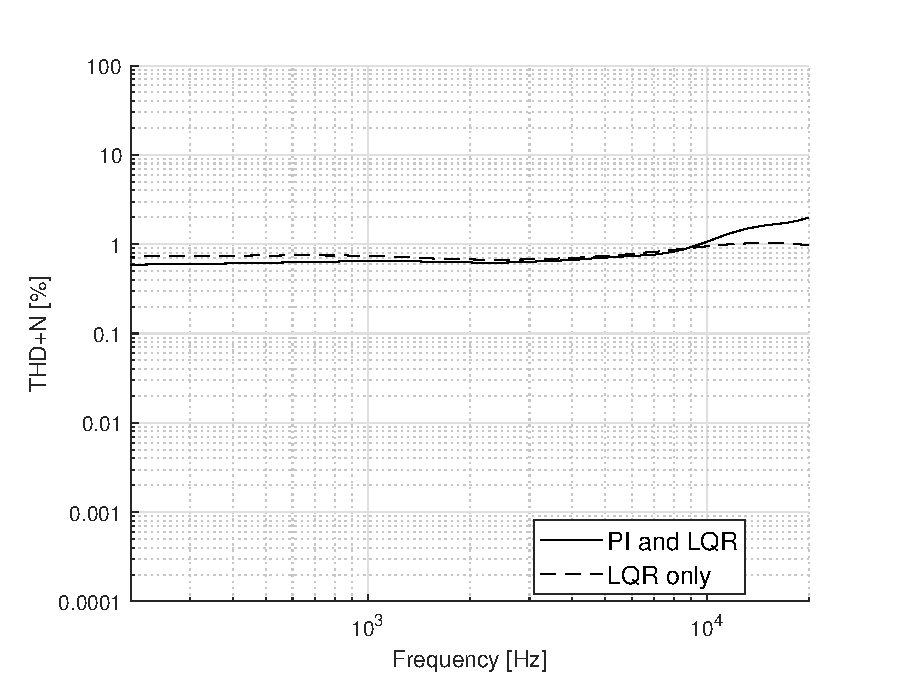
\includegraphics[width=0.8\textwidth]{Analysis/thdn.eps}
	\caption{THD+N of amplifier without and with feedback loop}
	\label{fig:thdn}
\end{figure}
Seen in \autoref{fig:thdn} is the measured THD+N from the measurement setup with APx500 Audio Analyzer \cite{apx500_user_manual} in \autoref{fig:apx500_typical_measurement}. In a practical sense, the analysis is performed by inputting a controlled sine wave sweep, filtering the output signal and comparing the ratio. This is described by the following expression:
\begin{equation} \label{eq:thdn_expression}
	\mathrm{THD+N} = \frac{\sum_{n=2}^{\infty} \mathrm{harmonics + noise}}{\mathrm{fundamental}}
\end{equation}
Seen in \autoref{eq:thdn_expression} is a mathematical expression of the calculation done by the audio analyzer. 
% Sæt mere ind omkring hvad man kan se. Måske lav nyt sweep og figur

\section{Control loop simulation}

\begin{figure}[htbp]
	\centering
	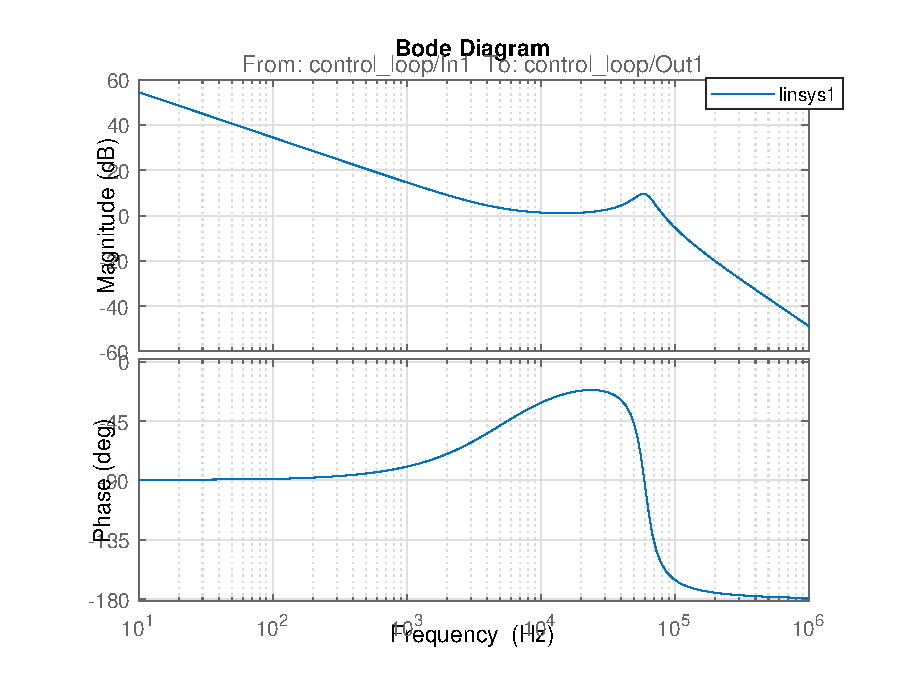
\includegraphics[width=0.8\textwidth]{Appendix/control_loop_figure_proper.eps}
	\caption{Control loop figure form Simulink}
	\label{fig:control_loop_figure_proper}
\end{figure}

\chapter{MATLAB code}
\lstinputlisting[basicstyle=\mlttfamily,caption=SimpleModulator.m,label={lst:simple_modulator.m},captionpos=t]{0_Figures/Appendix/PWM_modulation.m}

\begin{figure}[H]
	\centering
	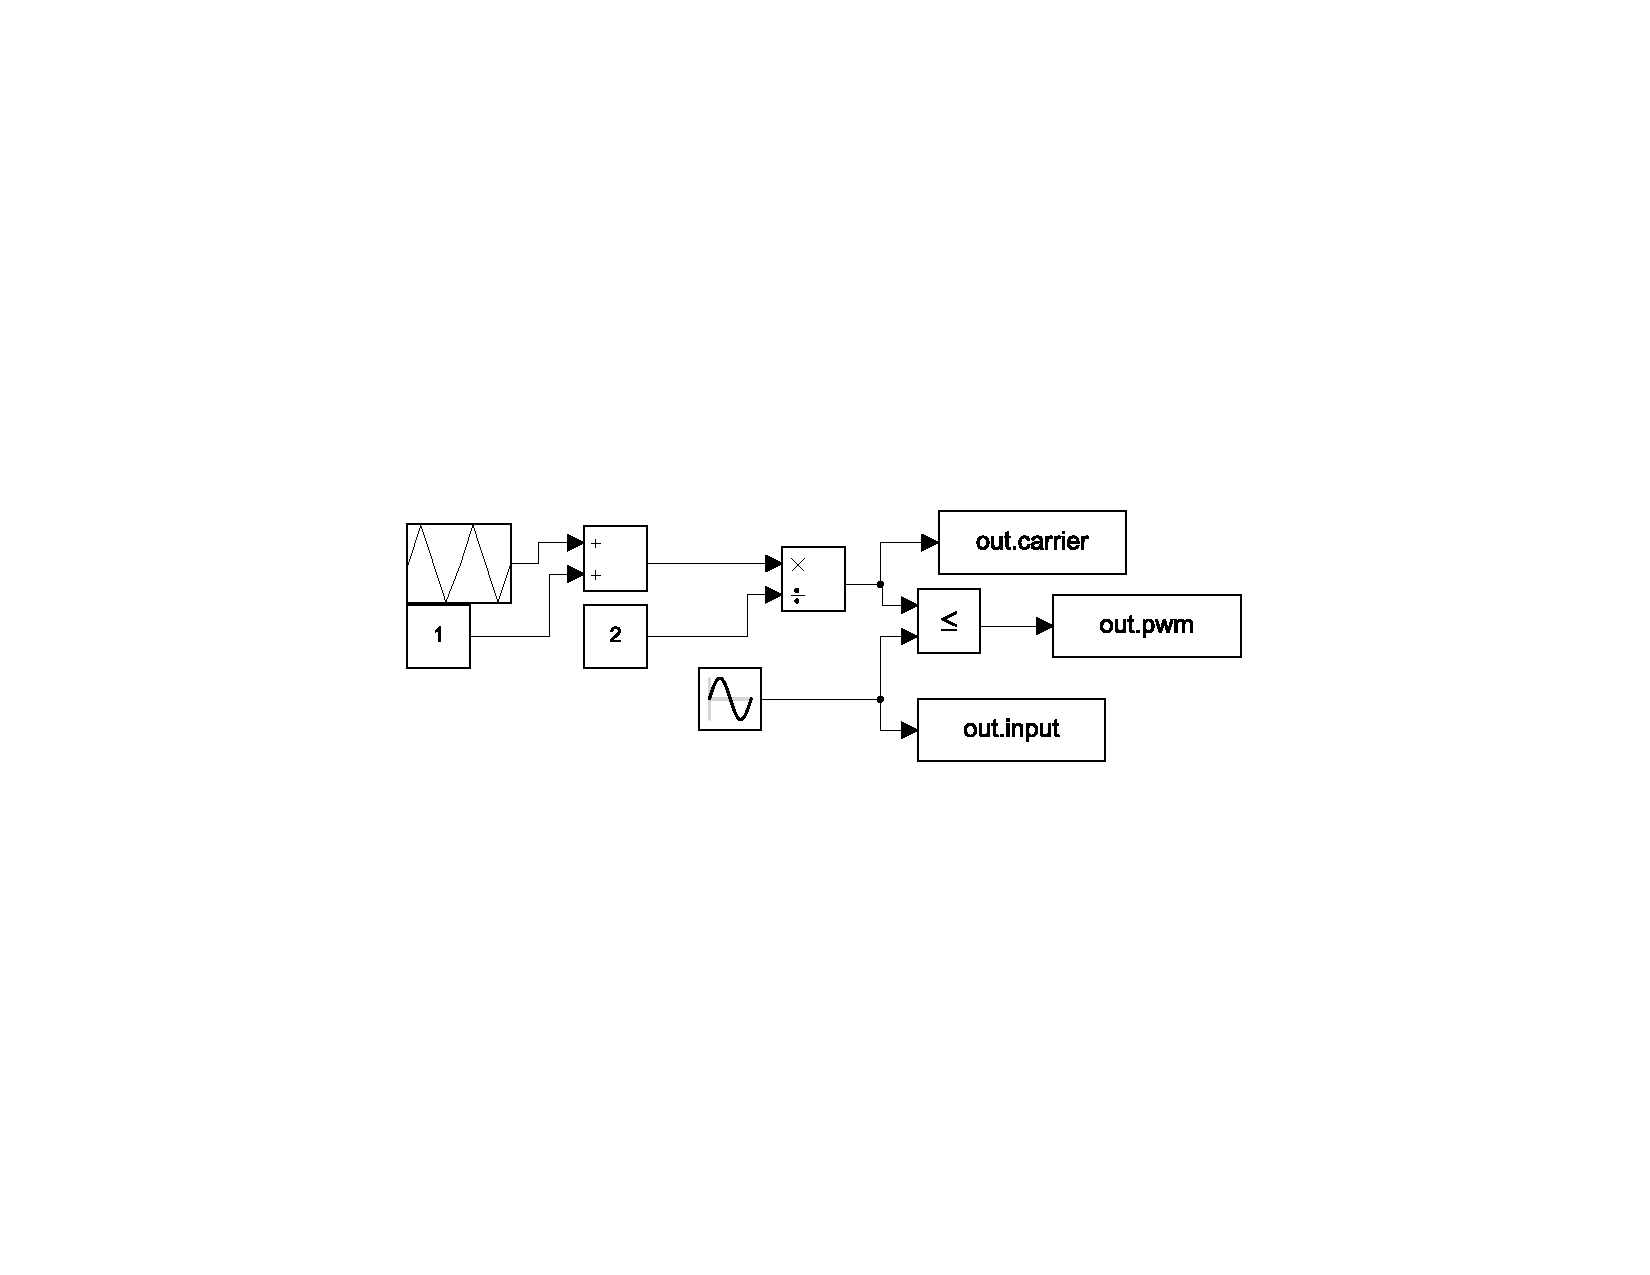
\includegraphics[width=0.9\textwidth,trim=100 200 100 200, clip]{Appendix/pwm_modulation_sim.pdf}
	\caption{Simulink model for a PWM generator}
	\label{fig:pwm_modulator_sim}
\end{figure}

\lstinputlisting[basicstyle=\mlttfamily,caption=Regulator Calculation.m,label={lst:lqi_designer},captionpos=t]{0_Figures/Appendix/LQI_Designer.m}

\lstinputlisting[basicstyle=\mlttfamily,caption=Inductor Design.m,label={lst:inductor_design2},captionpos=t]{0_Figures/Appendix/inductor_design2.m}

\lstinputlisting[basicstyle=\mlttfamily,caption=Simulation Script.m,label={lst:simulationLTspice.m},captionpos=t]{0_Figures/Appendix/Simulation_Master_Script.m}

\lstinputlisting[basicstyle=\mlttfamily,caption=sim matlab importer.m,label={lst:simmatlabimporter.m},captionpos=t]{0_Figures/Appendix/sim_matlab_importer.m}

\lstinputlisting[basicstyle=\mlttfamily,caption=bode100importer.m,label={lst:bode100importer.m},captionpos=t]{0_Figures/Appendix/bode100_importer_plot.m}

\lstinputlisting[basicstyle=\mlttfamily,caption=outputfilter.m,label={lst:outputfilter.m},captionpos=t]{0_Figures/Appendix/output_filter.m}

\lstinputlisting[basicstyle=\mlttfamily,caption=controlloop.m,label={lst:controlloop.m},captionpos=t]{0_Figures/Appendix/control_loop.m}

\chapter{Bill of Materials}
% Please add the following required packages to your document preamble:
% \usepackage{booktabs}
% \usepackage{multirow}
\begin{table}[H]
\adjustbox{max width=0.9\textwidth}{%
\centering
\begin{tabular}{@{}llllll@{}}
\toprule
\multicolumn{1}{c}{\textbf{Circuit}} & \textbf{Component} & \textbf{Value} & \textbf{Footprint} & \textbf{Rating} & \textbf{Description} \\ \midrule
\multirow{25}{*}{IO} & C1 & 1n & 0603 & X7R50V & Preamp \\
                   & C13 & 1u & RAD-0.3in & Film 40V & Preamp \\
                   & C14 & 1.5n & 0603 & X7R50V & PI controller \\
                   & C15 & NC & 0603 & X7R50V & PI controller \\
                   & C2,C3,C4,C9,C10 & 100n & 0603 & X7R16V & Decoupling \\
                   & C5,C11 & 1u & 0603 & X5R6.3V & Decoupling \\
                   & C6,C7 & 100n & 0805 & X7R50V & Decoupling \\
                   & C8 & 1500u & RAD-0.3in & 63Vdc & Decoupling \\
                   & P10 & 3-pin header & Male & 250V & Controller bypass \\
                   & P11,P12 & 10-pin header & Female & 250V & InterPCB con. \\
                   & P2,P3 & 1-pin header & Male & 250V & Measurements \\
                   & P4,P5 & 2-way screw & NA & 300V 15A & 30V Power,Output \\
                   & P6 & 2-pin header & Molex KK254 & 500V 4A & Audio in \\
                   & P7 & 4-pin header & Female & 250V & 5V Power \\
                   & P8,P9 & BNC & BNC PCB & 500V & Audio in, Output \\
                   & R2 & 16.2k & 0603 & 1\% & Preamp \\
                   & R1,R3 & 2k & 0603 & 1\% & Preamp \\
                   & R4,R7 & 4.75k & 0603 & 1\% & Voltage ref \\
                   & R5 & 33.2k & 0603 & NA & PI controller \\
                   & R6 & 0 (short) & 0603 & NA & PI controller \\
                   & R9 & 0 (short) & 0603 & NA & PI controller \\
                   & R10 & NC & 0603 & NA & PI controller \\
                   & R8 & 2.49k & 0603 & 1\% & Voltage ref \\
                   & U1 & OPA2365 & SOIC-8 & NA & Preamp, PI \\
                   & U2 & TLV431A & SOT-23 & 1\% & Voltage ref \\ \midrule
\multirow{14}{*}{Power Stage} & C1,C11,C15,C19 & 100n & 0603 & X7R16V & Gate driver \\
                   & P1,P2 & 10-pin header & Male & 250V & InterPCB con. \\
                   & C2,C16 & 150n & 0603 & X5R10V & Gate driver \\
                   & C3,C10 & 100p & 0603 & NPO50V & Decoupling \\
                   & L1,L2 & 1.768u & Radial & NA & Output filter \\
                   & U1,U3 & LM5113 & WSON-10 & NA & Gate driver \\
                   & R20 & 15m sense & 1210 & 1\% 1W & Output filter \\
                   & R1,R6 & 500 & SMDtrim 3213 & NA & Gate driver \\
                   & Q1,Q2,Q3,Q4 & BSZ097N10NS5 & TSDSON-8 & NA & Power stage \\
                   & R2,R5,R8,R10 & 5 & 0603 & 1\% & Gate driver \\
                   & R4,R9 & 0 & 0603 & 1\% & Gate driver \\
                   & D1,D2 & Diode & NA & 85V 0.25A & Gate driver \\
                   & C5,C6,C9,C17 & 10u & 1210 & X7R50V & Decoupling \\
                   & C12,C13,C14 & 680n & 1210 & X7R100V & Output filter \\ \midrule
\multirow{16}{*}{AIM+reg} & C18,C20,C27 & 100n & 0603 & X7R16V & Decoupling \\
                   & C28,C29,C30,C31 & 100n & 0603 & X7R16V & Decoupling \\
                   & U6 & LT1999 & MSOP-8 & NA & Current acq. \\
                   & U4 & AD8274 & MSOP-8 & NA & Volt acq. \\
                   & U2 & LT1711 & MSOP-8 & NA & AIM \\
                   & C4 & NC & 0603 & X7R16V & AIM \\
                   & C7 & NC & 0603 & X7R16V & AIM \\
                   & C8 & NC & 0603 & X7R16V & Cur. acq. \\
                   & CA1 & 1.5n & 0603 & X7R50V & AIM \\
                   & R14 & 8.66k & 0603 & 1\% & AIM \\
                   & R18 & 16.2k & 0603 & 1\% & AIM \\
                   & R23 & 1.5k & 0603 & 1\% & AIM \\
                   & R3,R11 & 120k & 0603 & 1\% & Voltage acq. \\
                   & RA1 & 2.2k & 0603 & 1\% & AIM \\
                   & RA2 & 20k & 0603 & 1\% & AIM \\
                   & RA3 & 2.74k & 0603 & 1\% & AIM \\
                   & RA4 & 0 & 0603 & NA & AIM \\ \bottomrule
\end{tabular}}
\caption{Bill of Materials}
\label{tab:bom}
\end{table}

\chapter{Instruments}
\begin{table}[H]
	\centering
	\begin{tabular}{@{}lll@{}}
		\toprule
		\textbf{Function} & \textbf{Manufacturer} & \textbf{Model} \\ \midrule
		Visual inspection microscope & Leica & A60 \\
		Manual soldering & Weller & WX2 \\
		Heat gun & Thermaltronics & TMT-HA600-2 \\
		SMT solder paste dispensing & Fisnar & SL101N \\
		Reflow oven & Mistral & 260 \\
		DMM & Meterman & 38XR \\ \bottomrule
	\end{tabular}
	\caption{List of instruments used for solder work}
	\label{tab:instruments_solder_work}
\end{table}

\begin{table}[H]
	\centering
	\begin{tabular}{@{}lll@{}}
		\toprule
		\textbf{Function} & \textbf{Manufacturer} & \textbf{Model} \\ \midrule
		Power supply & RIGOL & DP832 \\
		DMM & Agilent & 34410A \\
		Frequency response analysis & N4L & PSM1735 \\
		Audio analysis & Audio Precision & APx500 \\
		Audio analysis filter & Audio Precision & AUX-0025 \\
		Control loop analyzer & OMICRON Lab & BODE 100 \\
		Control loop injection transformer & OMICRON Lab & B-WIT 100 \\
		Passive load & Unknown & Power resistor \SI{4}{\ohm} \\
		Passive load & Unknown & Loudspeaker \SI{4}{\ohm} \\
		Active cooling & ebm & W2S107-AA01-16 \\ \bottomrule
	\end{tabular}
	\caption{List of instruments used for testing}
	\label{tab:instruments_hardware}
\end{table}
